\NeedRoom{10}

\subsection{Staged Investment and Implementation Gates}

\begin{figure}[htbp]\centering

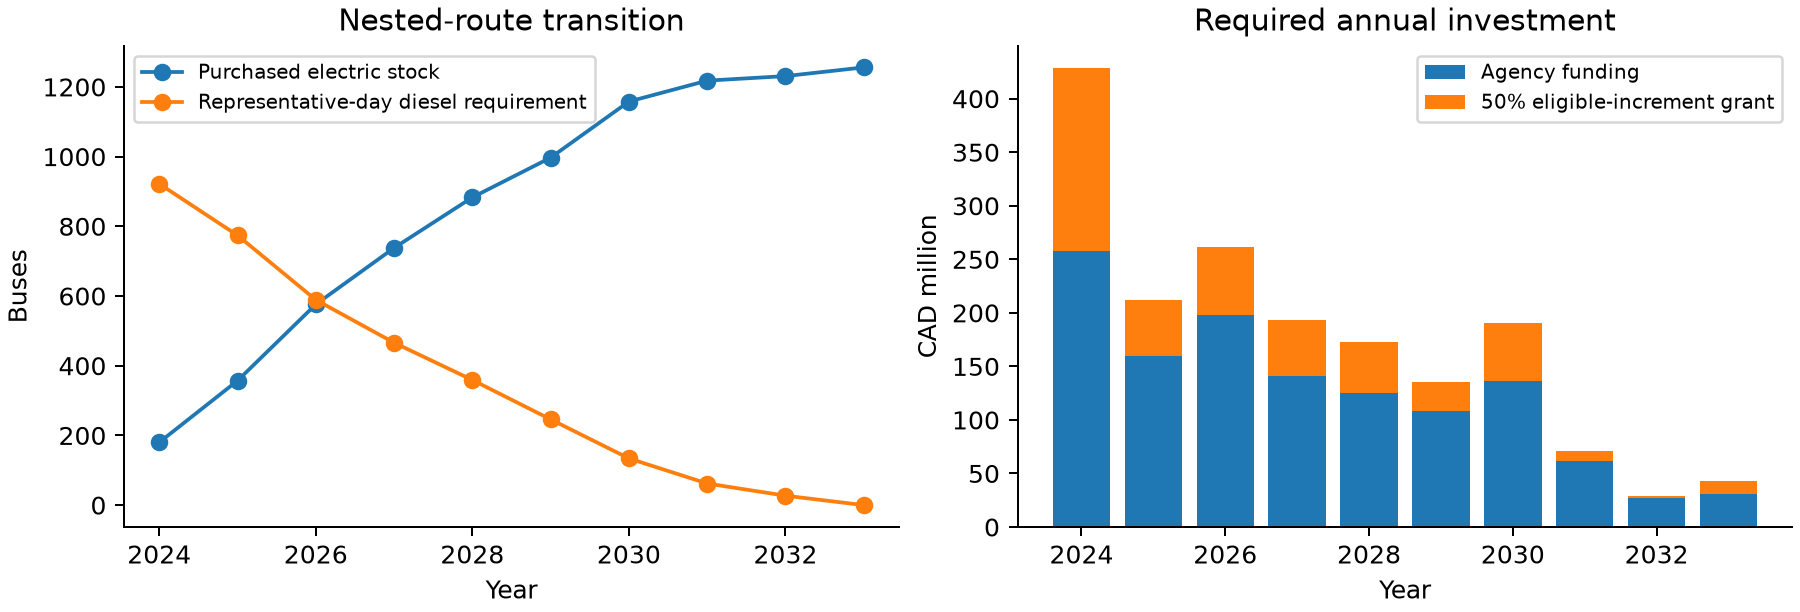
\includegraphics[width=\textwidth,height=0.37\textheight,keepaspectratio]{images/roadmap.png}

\caption{Purchased electric stock, representative-day residual diesel requirements, and annual required investment.}\label{fig:result4}

\end{figure}

\begin{longtable}{@{}L{\dimexpr 0.12000\textwidth-2\tabcolsep\relax}L{\dimexpr 0.21000\textwidth-2\tabcolsep\relax}L{\dimexpr 0.21000\textwidth-2\tabcolsep\relax}L{\dimexpr 0.21000\textwidth-2\tabcolsep\relax}L{\dimexpr 0.25000\textwidth-2\tabcolsep\relax}@{}}
\caption{Vancouver staged grants, agency capital and battery replacement (CAD million)}\label{tab:source12}\\
\toprule
\textbf{Year} & \textbf{Grant 25\%} & \textbf{Grant 50\%} & \textbf{Agency 50\%} & \textbf{Battery replace- ment} \\
\midrule
\endfirsthead
\multicolumn{5}{l}{Table \thetable\ (continued)}\\
\toprule
\textbf{Year} & \textbf{Grant 25\%} & \textbf{Grant 50\%} & \textbf{Agency 50\%} & \textbf{Battery replace- ment} \\
\midrule
\endhead
\midrule\multicolumn{5}{r}{Continued on next page}\\\endfoot
\bottomrule\endlastfoot
2024 & 85.0 & 170.1 & 258.2 & 0.0 \\
2025 & 26.0 & 52.1 & 159.8 & 0.0 \\
2026 & 31.7 & 63.4 & 198.1 & 0.0 \\
2027 & 25.9 & 51.7 & 141.3 & 0.0 \\
2028 & 23.6 & 47.3 & 125.1 & 0.0 \\
2029 & 13.2 & 26.5 & 108.7 & 0.0 \\
2030 & 27.3 & 54.5 & 136.1 & 0.0 \\
2031 & 4.6 & 9.2 & 61.6 & 0.0 \\
2032 & 0.9 & 1.8 & 27.3 & 13.7 \\
2033 & 5.7 & 11.4 & 31.1 & 13.1 \\
\end{longtable}

The staged budget counts first-stage infrastructure, new vehicles and subsequent battery replacements. Its annual eligible increment deducts a counterfactual diesel replacement allowance. It is separate from the immediate-replacement NPV experiment.


The staged 50\%-grant cash ledger ends at CAD 59.7 million, including operating savings and avoided diesel purchases. The staged production-minus-operating estimate ends at 875.4 kt CO$_2$e; this is a different boundary from the immediate-replacement ten-year total and must not be substituted for it.


Purchase releases should follow three gates: firm charging capacity commissioned; winter range and equal capacity validated on assigned routes; and actual vehicle ages and home depots reconciled with the route groups. These gates can change the illustrated order.

